%Chapter 5

\chapter{Transfer Learning with Natural Lottery Winners} % Chapter title
\label{ch:tl_lth} % For referencing the chapter elsewhere, use \autoref{ch:introduction} 


\section{Introduction}
\label{sec:intro}
The ``Lottery-Ticket-Hypothesis" (LTH) \cite{frankle2018lottery} states that within large randomly initialized neural networks there exist smaller sub-networks which, if trained from their initial weights, can perform just as well as the fully trained unpruned network from which they are extracted. This happens to be possible because the weights of these sub-networks seem to be particularly well initialized before training starts, therefore making these smaller architectures suitable for learning (see Fig \ref{fig:tickets_visualization} for an illustration). These sub-networks, i.e., the pruned structure together with their initial weights, are called winning tickets, as they appear to have won the initialization lottery. Since winning tickets only contain a very limited amount of parameters, they yield faster training, inference, and sometimes even better final performance than their larger over-parametrized counterparts \cite{frankle2018lottery,franklestabilizing}. So far, winning tickets are typically identified by an iterative procedure that cycles through several steps of network training and weight pruning, starting from a randomly initialized unpruned network. While simple and intuitive, the resulting algorithm, has unfortunately a high computational cost. Despite the fact that the resulting sparse networks can be trained efficiently and in isolation from their initial weights, the LTH idea has not yet led to more efficient solutions for training a sparse network, than existing pruning algorithms that all also require to first fully train an unpruned network \cite{han2015deep,molchanov2016pruning,dong2017learning,lin2017runtime,zhuang2018discrimination}.

\begin{figure*}[!htb]
\minipage{0.3\textwidth}
  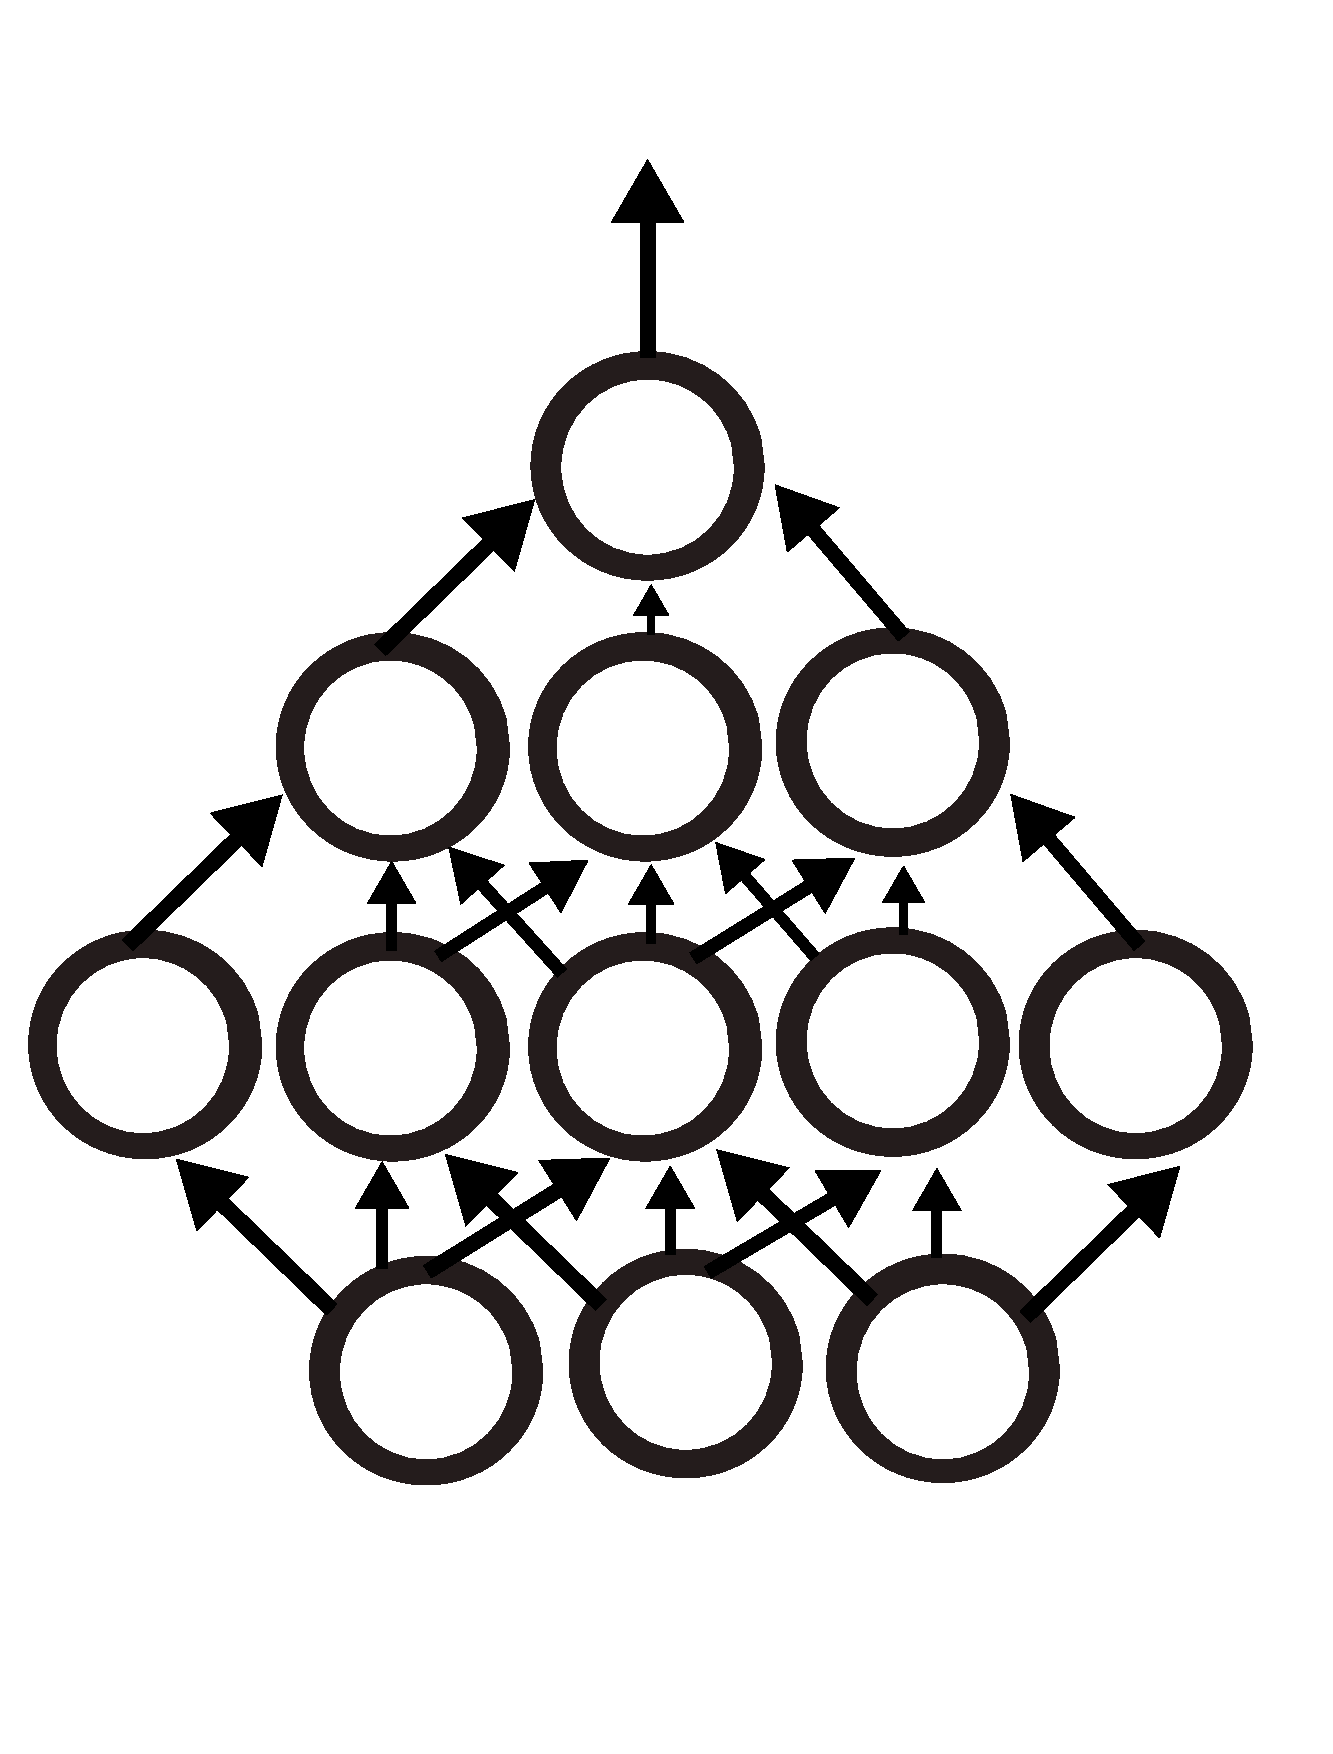
\includegraphics[width=\linewidth]{./Images/Chapter05/mlp.pdf}
\endminipage\hfill
\minipage{0.3\textwidth}
  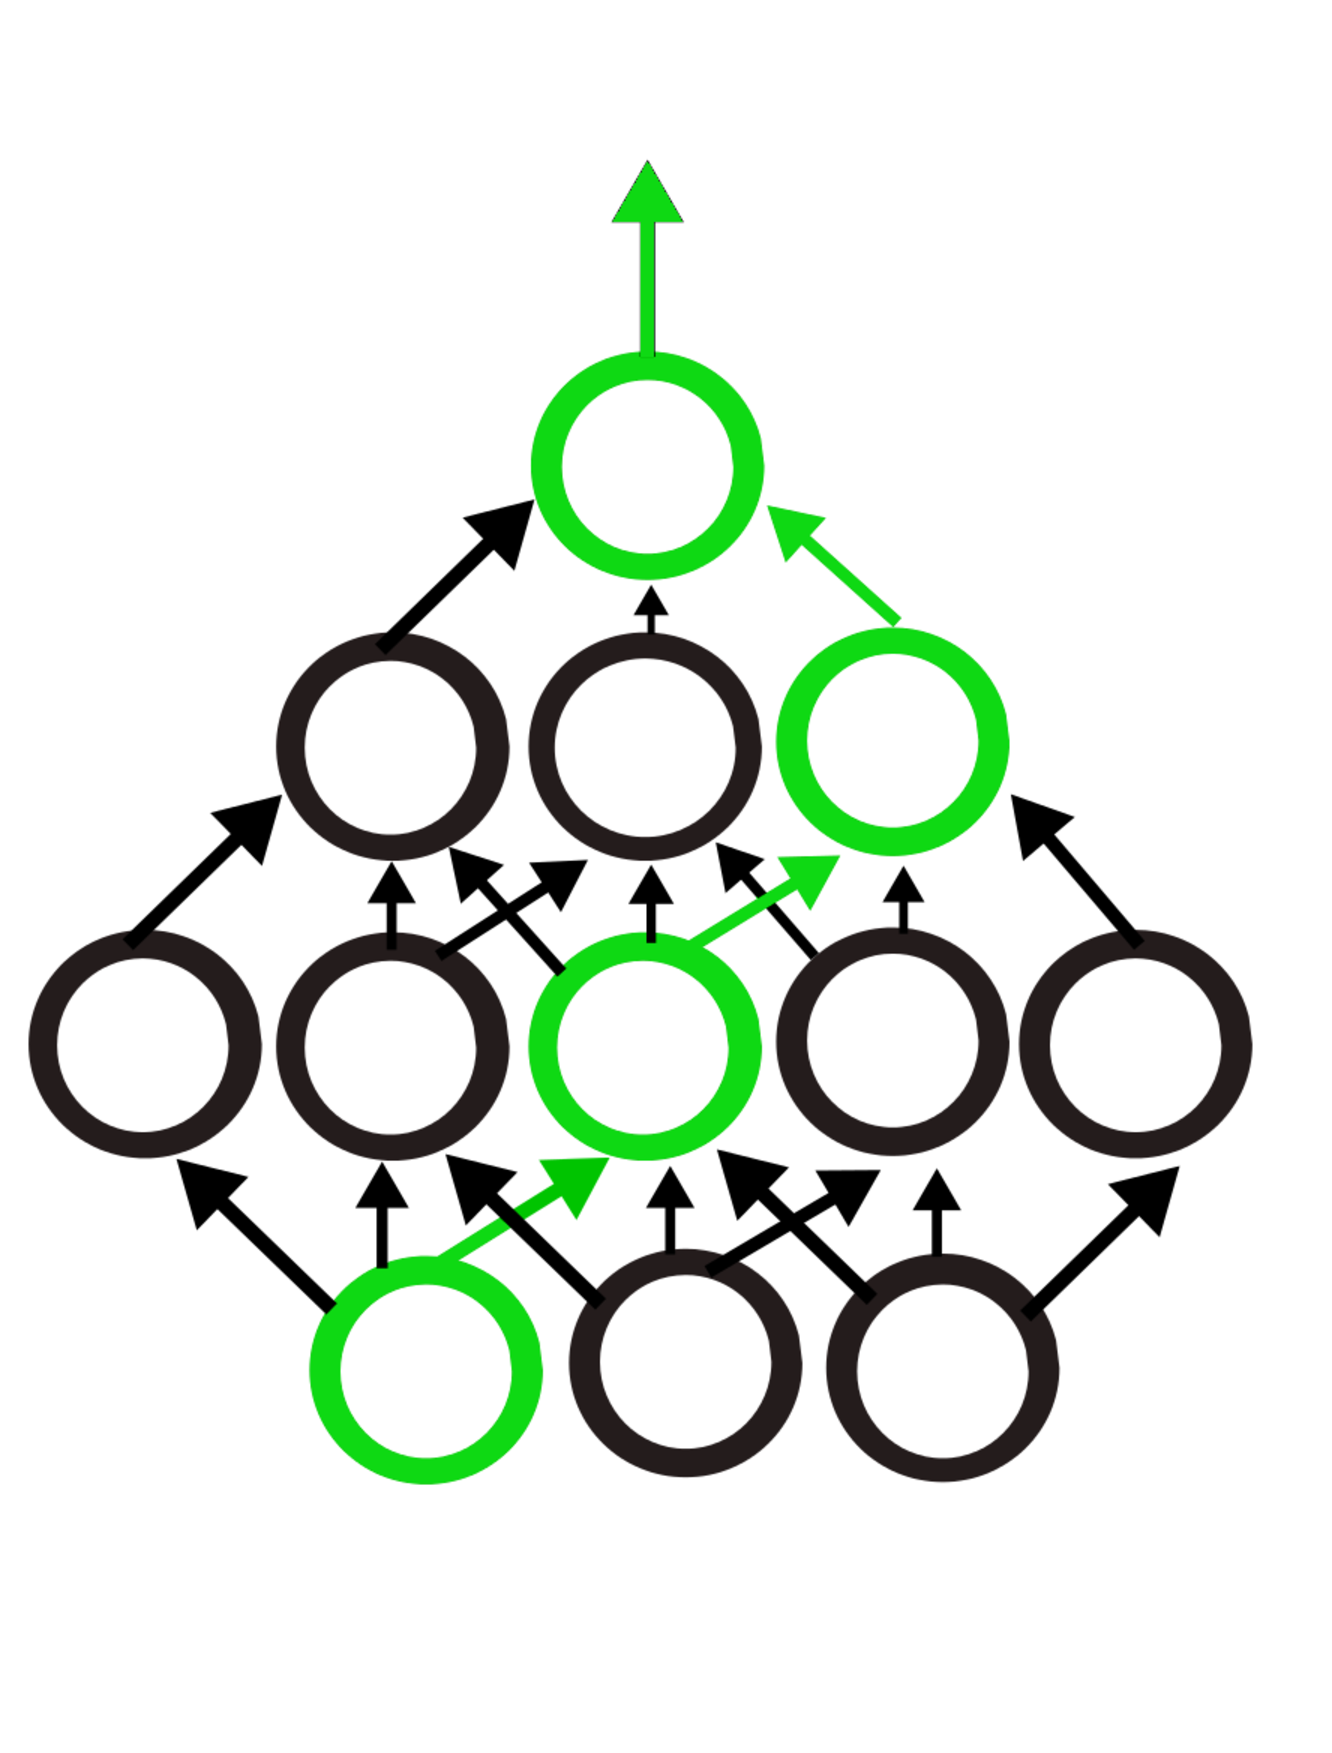
\includegraphics[width=\linewidth]{./Images/Chapter05/mlp_ticket_3.pdf}
\endminipage\hfill
\minipage{0.3\textwidth}%
  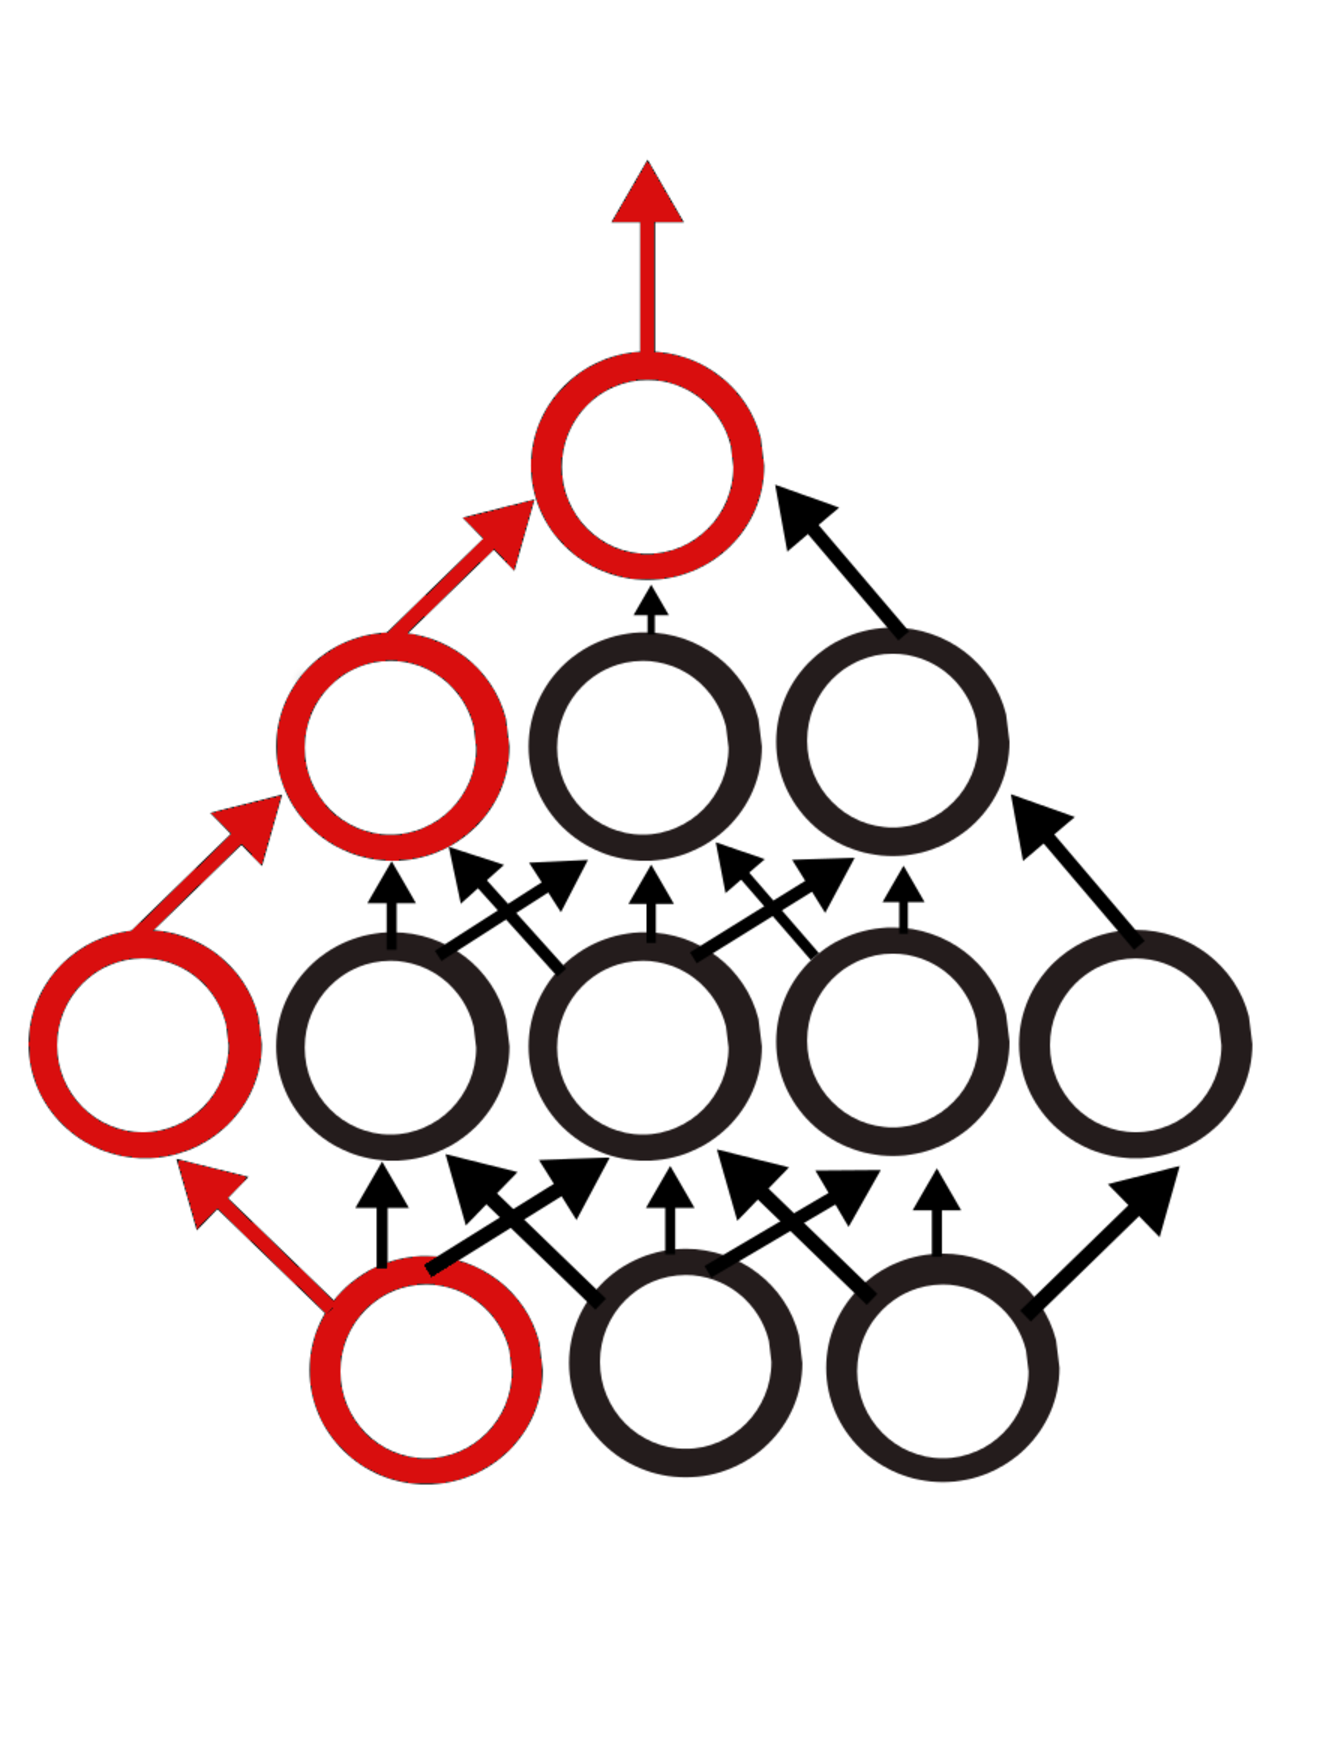
\includegraphics[width=\linewidth]{./Images/Chapter05/random_ticket_1.pdf}
\endminipage
\caption{A visual representation of the LTH as introduced in \cite{frankle2018lottery}. Let us consider a simplified version of a two hidden layer feedforward neural network as is depicted in the first image on the left. The LTH states that within this neural network there exist multiple smaller networks (represented in green), which perform just as well as their larger counterpart. Training these sparse models from scratch successfully is only possible as long as their weights are initialized with the same values that were also used when the larger (black) model was initialized. As can be seen by the blue curve of the last plot the performance of such pruned models gets barely harmed even when large pruning rates are reached. These models are considered as the winners of the initialization lottery and also perform better than the same models re-initialized randomly (orange line). Results obtained on the MNIST dataset that replicate the findings presented in \cite{frankle2018lottery}.}%
    \label{fig:tickets_visualization}%
\end{figure*}

\begin{figure}[ht]
  \centering
  \begin{tikzpicture}[scale = 0.8]

\begin{axis}[
	grid style={dashed,gray},
	grid = both, 
	tick style=black,
  	xlabel=Fraction of Weights Pruned,
  	ylabel= Accuracy ($\%$),
	title=CIFAR-10,
	%width=1,
	ymin=0,
    	ymax=85,
  	legend pos=outer north east,
]

	\addlegendentry{Baseline}
	\addlegendentry{Winning Ticket $f(x;m\odot\theta_k)$}
	\addlegendentry{Random Ticket $f(x;m\odot\theta_r)$}

\addplot [thick, black, mark=x] table [x=pruning_stages, y=baseline]{./Results/Chapter05/logs/cifar10_example.txt};
\addplot [thick, blue, mark=x] table [x=pruning_stages, y=ticket]{./Results/Chapter05/logs/cifar10_example.txt};
\addplot [thick, orange, mark=x] table [x=pruning_stages, y=random_weights]{./Results/Chapter05/logs/cifar10_example.txt};

\end{axis}
    \end{tikzpicture}

   \caption{}
    \label{fig:original_lth_results}
\end{figure} 


Since the introduction of the idea of the LTH, several research works have focused on understanding what makes some weights so special to be the winners of the initialization lottery. Among the different tested approaches, which will be reviewed in Sec. \ref{sec:related_work}, one research direction in particular has looked into how well winning ticket initializations can be transferred among different training settings (datasets and optimizers), an approach which aims at characterizing the winners of the LTH by studying to what extent their inductive biases are generic \cite{morcos2019one}. The most interesting findings of this study are that winning tickets generalize across datasets, within the natural image domain at least, and that tickets obtained from larger datasets typically generalize better. This opens the door to the transfer of winning tickets between datasets, which makes the high computational cost required to identify them much more acceptable practically, as this cost has to be paid only once and can be shared across datasets.

In this paper, we build on top of this latter work. While Morcos et al. \cite{morcos2019one} focused on the natural image domain, we investigate the possibility of transferring winning tickets obtained from the natural image domain to datasets in non natural image domains. This question has an important practical interest as datasets in non natural image domains are typically scarcer than datasets in natural image domains. They would therefore potentially benefit more from a successful transfer of sparse networks, since the latter can be expected to require less data for training than large over-parametrized networks. Furthermore, besides studying their generalization capabilities, we also focus on another interesting property that characterizes models that win the LTH, and which so far has received less research attention. As originally presented in \cite{frankle2018lottery}, pruned models which are the winners of the LTH can yield a final performance which is better than the one obtained by larger over-parametrized networks. In this work we explore whether it is worth seeking for such pruned models when training data is scarce, a scenario that is well known to constraint the training of deep neural networks. To answer these two questions, we carried out experiments on several datasets from two very different non natural image domains: digital pathology and digital heritage.

\textbf{Research questions and contributions:} this work investigates two research questions. First, we aim at better characterizing the LTH phenomenon by investigating whether lottery winners that are found on datasets of natural images contain inductive biases that are strong enough to allow them to generalize to non-natural image distributions. To do so, we present to the best of our knowledge the first results that study the transferability of winning initializations in this particular training setting. Second, we thoroughly study for the first time whether pruned models that are the winners of the LTH can consistently outperform their larger over-parametrized counterparts in conditions with scarce training data.
